\documentclass{ximera}

 

\usepackage{epsfig}

\graphicspath{
  {./}
  {figures/}
}

\usepackage{morewrites}
\makeatletter
\newcommand\subfile[1]{%
\renewcommand{\input}[1]{}%
\begingroup\skip@preamble\otherinput{#1}\endgroup\par\vspace{\topsep}
\let\input\otherinput}
\makeatother

\newcommand{\includeexercises}{\directlua{dofile("/home/jim/linearAlgebra/laode/exercises.lua")}}

%\newcounter{ccounter}
%\setcounter{ccounter}{1}
%\newcommand{\Chapter}[1]{\setcounter{chapter}{\arabic{ccounter}}\chapter{#1}\addtocounter{ccounter}{1}}

%\newcommand{\section}[1]{\section{#1}\setcounter{thm}{0}\setcounter{equation}{0}}

%\renewcommand{\theequation}{\arabic{chapter}.\arabic{section}.\arabic{equation}}
%\renewcommand{\thefigure}{\arabic{chapter}.\arabic{figure}}
%\renewcommand{\thetable}{\arabic{chapter}.\arabic{table}}

%\newcommand{\Sec}[2]{\section{#1}\markright{\arabic{ccounter}.\arabic{section}.#2}\setcounter{equation}{0}\setcounter{thm}{0}\setcounter{figure}{0}}

\newcommand{\Sec}[2]{\section{#1}}

\setcounter{secnumdepth}{2}
%\setcounter{secnumdepth}{1} 

%\newcounter{THM}
%\renewcommand{\theTHM}{\arabic{chapter}.\arabic{section}}

\newcommand{\trademark}{{R\!\!\!\!\!\bigcirc}}
%\newtheorem{exercise}{}

\newcommand{\dfield}{{\sf dfield9}}
\newcommand{\pplane}{{\sf pplane9}}

\newcommand{\EXER}{\section*{Exercises}}%\vspace*{0.2in}\hrule\small\setcounter{exercise}{0}}
\newcommand{\CEXER}{}%\vspace{0.08in}\begin{center}Computer Exercises\end{center}}
\newcommand{\TEXER}{} %\vspace{0.08in}\begin{center}Hand Exercises\end{center}}
\newcommand{\AEXER}{} %\vspace{0.08in}\begin{center}Hand Exercises\end{center}}

% BADBAD: \newcommand{\Bbb}{\bf}

\newcommand{\R}{\mbox{$\Bbb{R}$}}
\newcommand{\C}{\mbox{$\Bbb{C}$}}
\newcommand{\Z}{\mbox{$\Bbb{Z}$}}
\newcommand{\N}{\mbox{$\Bbb{N}$}}
\newcommand{\D}{\mbox{{\bf D}}}
\usepackage{amssymb}
%\newcommand{\qed}{\hfill\mbox{\raggedright$\square$} \vspace{1ex}}
%\newcommand{\proof}{\noindent {\bf Proof:} \hspace{0.1in}}

\newcommand{\setmin}{\;\mbox{--}\;}
\newcommand{\Matlab}{{M\small{AT\-LAB}} }
\newcommand{\Matlabp}{{M\small{AT\-LAB}}}
\newcommand{\computer}{\Matlab Instructions}
\newcommand{\half}{\mbox{$\frac{1}{2}$}}
\newcommand{\compose}{\raisebox{.15ex}{\mbox{{\scriptsize$\circ$}}}}
\newcommand{\AND}{\quad\mbox{and}\quad}
\newcommand{\vect}[2]{\left(\begin{array}{c} #1_1 \\ \vdots \\
 #1_{#2}\end{array}\right)}
\newcommand{\mattwo}[4]{\left(\begin{array}{rr} #1 & #2\\ #3
&#4\end{array}\right)}
\newcommand{\mattwoc}[4]{\left(\begin{array}{cc} #1 & #2\\ #3
&#4\end{array}\right)}
\newcommand{\vectwo}[2]{\left(\begin{array}{r} #1 \\ #2\end{array}\right)}
\newcommand{\vectwoc}[2]{\left(\begin{array}{c} #1 \\ #2\end{array}\right)}

\newcommand{\ignore}[1]{}


\newcommand{\inv}{^{-1}}
\newcommand{\CC}{{\cal C}}
\newcommand{\CCone}{\CC^1}
\newcommand{\Span}{{\rm span}}
\newcommand{\rank}{{\rm rank}}
\newcommand{\trace}{{\rm tr}}
\newcommand{\RE}{{\rm Re}}
\newcommand{\IM}{{\rm Im}}
\newcommand{\nulls}{{\rm null\;space}}

\newcommand{\dps}{\displaystyle}
\newcommand{\arraystart}{\renewcommand{\arraystretch}{1.8}}
\newcommand{\arrayfinish}{\renewcommand{\arraystretch}{1.2}}
\newcommand{\Start}[1]{\vspace{0.08in}\noindent {\bf Section~\ref{#1}}}
\newcommand{\exer}[1]{\noindent {\bf \ref{#1}}}
\newcommand{\ans}{}
\newcommand{\matthree}[9]{\left(\begin{array}{rrr} #1 & #2 & #3 \\ #4 & #5 & #6
\\ #7 & #8 & #9\end{array}\right)}
\newcommand{\cvectwo}[2]{\left(\begin{array}{c} #1 \\ #2\end{array}\right)}
\newcommand{\cmatthree}[9]{\left(\begin{array}{ccc} #1 & #2 & #3 \\ #4 & #5 &
#6 \\ #7 & #8 & #9\end{array}\right)}
\newcommand{\vecthree}[3]{\left(\begin{array}{r} #1 \\ #2 \\
#3\end{array}\right)}
\newcommand{\cvecthree}[3]{\left(\begin{array}{c} #1 \\ #2 \\
#3\end{array}\right)}
\newcommand{\cmattwo}[4]{\left(\begin{array}{cc} #1 & #2\\ #3
&#4\end{array}\right)}

\newcommand{\Matrix}[1]{\ensuremath{\left(\begin{array}{rrrrrrrrrrrrrrrrrr} #1 \end{array}\right)}}

\newcommand{\Matrixc}[1]{\ensuremath{\left(\begin{array}{cccccccccccc} #1 \end{array}\right)}}



\renewcommand{\labelenumi}{\theenumi)}
\newenvironment{enumeratea}%
{\begingroup
 \renewcommand{\theenumi}{\alph{enumi}}
 \renewcommand{\labelenumi}{(\theenumi)}
 \begin{enumerate}}
 {\end{enumerate}\endgroup}



\newcounter{help}
\renewcommand{\thehelp}{\thesection.\arabic{equation}}

%\newenvironment{equation*}%
%{\renewcommand\endequation{\eqno (\theequation)* $$}%
%   \begin{equation}}%
%   {\end{equation}\renewcommand\endequation{\eqno \@eqnnum
%$$\global\@ignoretrue}}

%\input{psfig.tex}

\author{Martin Golubitsky and Michael Dellnitz}

%\newenvironment{matlabEquation}%
%{\renewcommand\endequation{\eqno (\theequation*) $$}%
%   \begin{equation}}%
%   {\end{equation}\renewcommand\endequation{\eqno \@eqnnum
% $$\global\@ignoretrue}}

\newcommand{\soln}{\textbf{Solution:} }
\newcommand{\exercap}[1]{\centerline{Figure~\ref{#1}}}
\newcommand{\exercaptwo}[1]{\centerline{Figure~\ref{#1}a\hspace{2.1in}
Figure~\ref{#1}b}}
\newcommand{\exercapthree}[1]{\centerline{Figure~\ref{#1}a\hspace{1.2in}
Figure~\ref{#1}b\hspace{1.2in}Figure~\ref{#1}c}}
\newcommand{\para}{\hspace{0.4in}}

\renewenvironment{solution}{\suppress}{\endsuppress}

\ifxake
\newenvironment{matlabEquation}{\begin{equation}}{\end{equation}}
\else
\newenvironment{matlabEquation}%
{\let\oldtheequation\theequation\renewcommand{\theequation}{\oldtheequation*}\begin{equation}}%
  {\end{equation}\let\theequation\oldtheequation}
\fi

\makeatother


\title{A Single Differential Equation}

\begin{document}
\begin{abstract}
\end{abstract}
\maketitle

  \label{S:growthmodels}

Algebraic operations such as addition and multiplication are
performed on numbers while the calculus operations of
differentiation and integration are performed on functions.
Thus algebraic equations (such as $x^2=9$) are solved for
numbers ($x=\pm 3$) while differential (and integral) equations
are solved for functions.

In Chapter~\ref{lineq} we discussed how to solve systems of
linear equations, such as
\begin{eqnarray*}
x_1 + x_2 & = & 2 \\
x_1 - x_2 & = & 4
\end{eqnarray*}
for numbers
\[
x_1=3 \quad \mbox{ and } \quad x_2=-1,
\]
while in this chapter we discuss how to solve some systems of
differential equations for functions.

Solving a single linear equation in one unknown $x$ is a simple
task.  For example, solve
\[
2x = 4
\]
for $x=2$.  Solving a single differential equation in one unknown function
$x(t)$ is far from trivial.

\subsubsection*{Integral Calculus as a Differential Equation}
\index{integral calculus}

Mathematically, the simplest type of differential equation is:
\begin{equation} \label{e:intcalc}
\dps\frac{dx}{dt}(t) = f(t)
\end{equation}
where $f$ is some continuous function.  In words, this equation asks us
to find all functions $x(t)$ whose derivative is $f(t)$.  The fundamental
theorem of calculus tells us the answer: $x(t)$ is an antiderivative of
$f(t)$.  Thus to find all solutions, we just integrate both sides of
\eqref{e:intcalc} with respect to $t$.  Formally, using indefinite integrals, 
\begin{equation}  \label{E:integrate}
\int \frac{dx}{dt}(t)dt = \int f(t)dt + C,
\end{equation}
where $C$ is an arbitrary constant.  (It is tempting to put a constant of
integration on both sides of \eqref{E:integrate}, but two constants are not 
needed, as we can just combine both constants on the right hand side of
this equation.)   Since the indefinite integral of $dx/dt$ is just the
function $x(t)$, we have 
\begin{equation}  \label{e:intcalcsoln}
x(t) = \int f(\tau) d\tau + C.
\end{equation}
In particular, finding closed form solutions to differential equations
of the type \eqref{e:intcalc} is equivalent to finding all definite
integrals of the function $f(t)$.  Indeed, to find closed form solutions 
to differential equations like \eqref{e:intcalc} we need to know all of the 
techniques of integration from integral calculus.

We note that if $x(t)$ is a real-valued function of $t$, then we denote the 
derivative of $x$ with respect to $t$ using the following
\[
\frac{dx}{dt}\qquad \dot{x} \qquad x'
\]
all of which are standard notations for the derivative.


\subsubsection*{Initial Conditions and the Role of the Integration Constant 
$C$}

Equation \eqref{e:intcalcsoln} tells us that there are an infinite number of
solutions to the differential equation \eqref{e:intcalc}, each one
corresponding to a different choice of the constant $C$.  To understand how
to interpret the constant $C$, consider the example
\[
\dps\frac{dx}{dt}(t) = \cos t.
\]
Using \eqref{e:intcalcsoln} we see that the answer is
\[
x(t) = \int \cos\tau d\tau  + C = \sin t + C.
\]
Note that 
\[
x(0) = \sin(0) + C = C.
\]
Thus, the constant $C$ represents an {\em initial condition\/} for the  
differential equation.  We will return to the discussion of initial 
conditions several times in this chapter.

See Exercise~\ref{c3.1.7} for a more interesting example of this type of
differential equation.

\subsubsection*{Solutions to Differential Equations are Functions}

Consider the differential equation \index{differential equation}
\begin{equation} \label{E:verify}
\frac{dx}{dt}(t) = tx(t).
\end{equation}
Are the functions
\[
x_1(t) = t^2 \AND x_2(t) = e^{t^2/2}
\]
solutions to the differential equation \eqref{E:verify}?

To test whether or not the function $x_1(t)$ is a solution, we compute
the left and right hand sides of \eqref{E:verify}:
\begin{eqnarray*}
{\rm LHS:} & \frac{d}{dt}x_1(t) & = 2t\\
{\rm RHS:} &  tx_1(t) & = t^3.
\end{eqnarray*}
Since the left and right hand sides are unequal, the function $x_1(t)$
is not a solution to \eqref{E:verify}.

To test whether or not the function $x_2(t)$ is a solution, we again
compute the left and right hand sides of \eqref{E:verify}:
\begin{eqnarray*}
{\rm LHS:} & \frac{d}{dt}x_2(t) & = te^{t^2/2}\\
{\rm RHS:} &  tx_2(t) & = te^{t^2/2}.
\end{eqnarray*}
Since the left and right hand sides are equal, the function $x_2(t)$
is a solution to \eqref{E:verify}.

Note that we have not discussed how we knew that the function $x_2(t)$
is a solution to \eqref{E:verify}.  For the most part, the issue of how
one finds solutions to a differential equation will be discussed in later
chapters, though we do determine solutions to a very important equation next.

\subsubsection*{The Linear Differential Equation of Growth and Decay}

The real subject of differential equations begins when the function $f$
on the right hand side of \eqref{e:intcalc} depends explicitly on the
function $x$, and the simplest such differential equation is:
\[
\frac{dx}{dt}(t) = x(t).
\]
Using results from calculus, we can solve this equation; indeed,
we can solve the slightly more complicated equation
\begin{equation}  \label{lin1}
\frac{dx}{dt}(t) = \lambda x(t),
\end{equation}
where $\lambda\in\R$ is a constant.  The differential equation \eqref{lin1} is 
{\em linear\/} since $x(t)$ appears by itself on the right hand side.  
Moreover, \eqref{lin1} is {\em homogeneous\/} since the constant function 
$x(t)=0$ is a solution.


In words \eqref{lin1} asks: For which functions $x(t)$ is the
derivative of $x(t)$ a scalar multiple of $x(t)$.  The function
\[
x(t)=e^{\lambda t}
\]
is such a function, since
\[
\frac{dx}{dt}(t) = \frac{d}{dt}e^{\lambda t} =
\lambda e^{\lambda t} = \lambda x(t).
\]
More generally, the function
\begin{equation} \label{soln1}
x(t) = K e^{\lambda t}
\end{equation}
is a solution to \eqref{lin1} for any real constant $K$.  We claim
that the functions \eqref{soln1} list all (differentiable)
functions that solve \eqref{lin1}.

To verify this claim, we let $x(t)$ be a solution to \eqref{lin1}
and show that the ratio 
\[
\frac{x(t)}{e^{\lambda t}} = x(t)e^{-\lambda t}
\]
is a constant (independent of $t$).  Using the product rule 
\index{product rule} and \eqref{lin1}, compute
\begin{eqnarray*}
\frac{d}{dt}\left[x(t)e^{-\lambda t}\right] & = &
\frac{d}{dt}\left(x(t)\right) e^{-\lambda t} +
x(t)\frac{d}{dt}\left(e^{-\lambda t}\right) \\
& = &
(\lambda x(t)) e^{-\lambda t} + x(t)(-\lambda e^{-\lambda t}) \\
& = & 0.
\end{eqnarray*}
Now recall that the only functions whose derivatives are
identically zero are the constant functions.  Thus,
\[
x(t) e^{-\lambda t} = K
\]
for some constant $K\in\R$.  Hence $x(t)$ has the form
\eqref{soln1}, as claimed.

Next, we discuss the role of the constant $K$.  We have written
the function as $x(t)$, and we have meant the reader to think of
the variable $t$ as time.  Thus $x(0)$ is the initial value of
the function $x(t)$ at time $t=0$; we say that $x(0)$ is the
{\em initial value\/}\index{initial value problem} of $x(t)$.
From \eqref{soln1} we see that
\[
x(0) = K,
\]
and that $K$ is the initial value of the solution of \eqref{lin1}.
Henceforth, we write $K$ as $x_0$ so that the notation calls
attention to the special meaning of this constant.

By deriving \eqref{soln1} we have proved:
\begin{theorem}  \label{T:singleeqn}
There is a unique solution to the {\em initial value problem\/}
\index{initial value problem}
\arraystart
\begin{equation} \label{ivp1}
\begin{array}{rcl}
\dps \frac{dx}{dt}(t) & = & \lambda x(t) \\
x(0) & = & x_0.
\end{array}
\end{equation}
\arrayfinish
That solution is
\[
x(t) = x_0e^{\lambda t}.
\]
\end{theorem}

As a consequence of Theorem~\ref{T:singleeqn} we see that there
is a qualitative difference in the behavior of solutions to
\eqref{ivp1} depending on whether $\lambda>0$ or $\lambda<0$.
Suppose that $x_0>0$.  Then
\begin{equation}  \label{explimits}
\lim_{t\to\infty} x(t) = \lim_{t\to\infty} x_0e^{\lambda t} =\left\{
\begin{array}{rl} +\infty & \quad\lambda>0 \\ 0 & \quad\lambda<0 . \end{array}
\right.
\end{equation}
When $\lambda>0$ we say that the solution has {\em exponential
growth\/}\index{exponential!growth} and when $\lambda< 0$ we say
that the solution has {\em exponential decay\/}
\index{exponential!decay}.  In either case, however, the
number $\lambda$ is called the {\em growth rate\/}\index{growth
rate}.  We can visualize this discussion by graphing the
solutions in \Matlabp.

Suppose we set $x_0=1$ and $\lambda=\pm 0.5$.  Type
\begin{verbatim}
x0 = 1;
lambda = 0.5;
t = linspace(-1,4,100);
x = x0*exp(lambda*t);
plot(t,x)
hold on
xlabel('t')
ylabel('x')
lambda = -0.5;
x = x0*exp(lambda*t);
plot(t,x)
\end{verbatim}
The result of this calculation is shown in
Figure~\ref{graph_labelfig}.  In this way we can actually see
the difference between exponential growth ($\lambda=0.5$) and
exponential decay ($\lambda=-0.5$), as discussed in
\eqref{explimits}.

\begin{figure}[htb]
     \centerline{%
     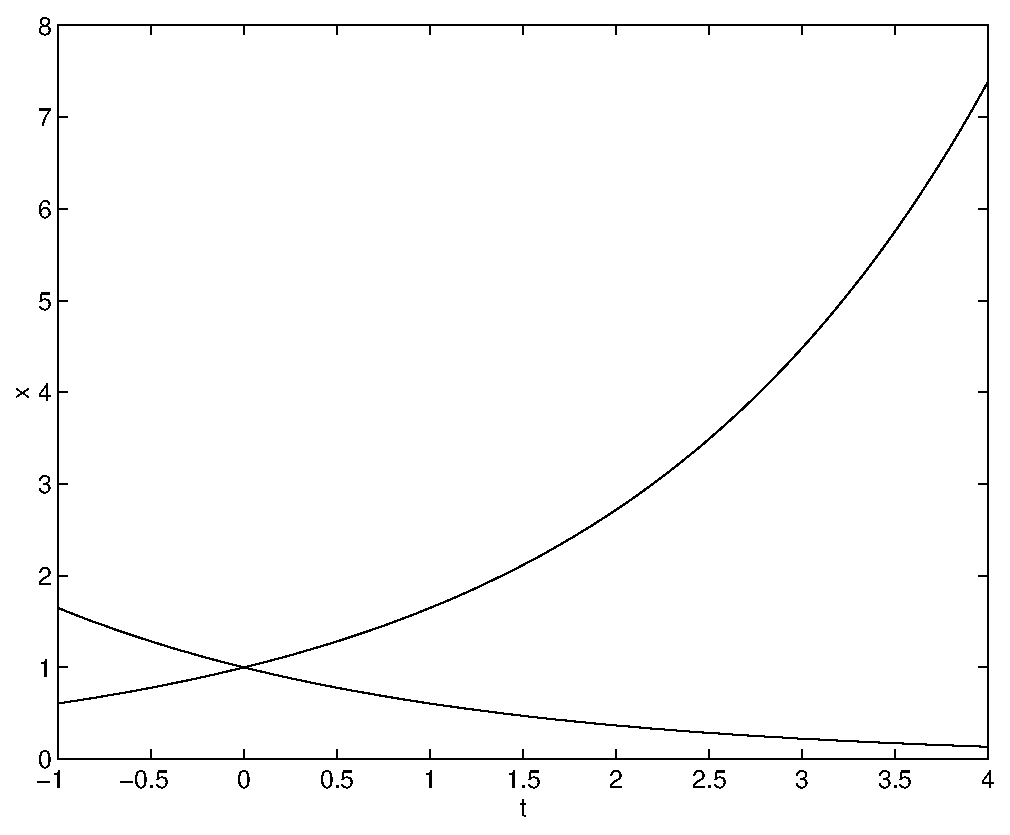
\psfig{file=../figures/graph1.eps,width=3.5in}}
     \caption{Solutions of \protect\eqref{lin1}
              for $t\in [-1,4]$, $x_0=1$ and $\lambda=\pm 0.5$.}
     \label{graph_labelfig}
\end{figure}


  \subsubsection*{The Inhomogeneous Linear Differential Equation}

It follows from \eqref{explimits} that solutions to the linear homogeneous
differential equation \eqref{ivp1} are either unbounded as $t\to \infty$ or 
they approach zero.  Now we consider an inhomogeneous differential 
equation and show that solutions can approach fixed values for increasing 
$t$ that are neither zero nor infinity.

As an example, consider the linear differential equation
\begin{equation} \label{E:ivp2}
\frac{dx}{dt} = -2x-6.
\end{equation}
Observe that $x(t)=0$ is not a solution of \eqref{E:ivp2} and therefore
that \eqref{E:ivp2} is {\em inhomogeneous}.  It is easy to verify, however, 
that the constant function $x(t)=-3$ is a solution.

Equation~\eqref{E:ivp2} can be solved by introducing a new function that 
transforms \eqref{E:ivp2} into a homogeneous equation.  Let
\[
y(t) = x(t) + 3,
\]
and compute
\[
\frac{dy}{dt} = \frac{dx}{dt} = -2x-6 = -2y.
\]

Using Theorem~\ref{T:singleeqn}, it follows that $y(t)$ has the form
\[
y(t) = y_0e^{-2t}.
\]
Therefore
\[
x(t) =  y_0e^{-2t}-3
\]
is a solution of \eqref{E:ivp2} for every constant $y_0$.  Moreover, 
\[
\lim_{t\to\infty} x(t) = \lim_{t\to\infty} y_0e^{-2t} -3=-3,
\]
which is neither zero nor infinity.

Any equation of the form
\begin{equation} \label{ivp2}
\frac{dx}{dt}(t)  = \lambda x(t) +\rho
\end{equation}
can be solved in a similar fashion.  Just set 
\[
y(t) = x(t) + \frac{\rho}{\lambda}.
\]
It follows from \eqref{ivp2} that
\[
\frac{dy}{dt} = \frac{dx}{dt} = \lambda x(t) +\rho =
\lambda\left( y(t)-\frac{\rho}{\lambda}\right) +\rho = \lambda y(t).
\]
Theorem~\ref{T:singleeqn} implies that $y(t) = y_0e^{\lambda t}$ for some 
constant $y_0$ and
\[
x(t) = y_0e^{\lambda t} - \frac{\rho}{\lambda}.
\]
Note that the limit of $x(t)$ as $t\to\infty$ is $-\rho/\lambda$ when 
$\lambda<0$.



\subsection*{Some Examples of \protect\eqref{ivp1}}

Even though the differential equation \eqref{lin1} is one of the
simplest differential equations, it still has some use in applications.
We present two here: compound interest and population dynamics.

\subsubsection*{Compound Interest} \index{compound interest}

Banks pay interest on an account in the following way.  At the
end of each day, the bank determines the interest rate $r_{day}$ for
that day, checks the principal $P$ in the account, and then
deposits an additional $r_{day}P$.  So the next day the principal in
this account is $(1+r_{day})P$.  Note that if $r$ denotes the
interest rate per year, then $r_{day} = r/365$.  Of course, a day
is just a convenient measure for elapsed time.  Before computers
were prevalent, banks paid interest yearly or quarterly or monthly
or, in a few cases, even weekly, depending on the particular bank rules.

Observe that the more frequently interest is paid, the more
money is earned. For example, if interest is paid only once at
the end of a year, then the money in the account at the end of
the year is $(1+r)P$, and the amount $rP$ is called {\em simple
interest\/}.  But if interest is paid twice a year, then the principal
at the end of six months will be $(1+\frac{r}{2})P$, and the principal
at the end of the year will be $(1+\frac{r}{2})^2P$.  Since
\[
\left(1+\frac{r}{2}\right)^2 = 1+r+\frac{1}{4}r^2 > 1+r,
\]
there is more money in the account at the end of the
year if the interest is compounded semiannually rather than
annually.  But how much is the difference and what is the
maximum earning potential?

While making the calculation in the previous paragraph, we
implicitly made a number of simplifying assumptions.  In
particular, we assumed
\begin{itemize}
\item	an initial principal $P_0$ is deposited in the bank on January 1,
\item	the money is not withdrawn for one year,
\item	no new money is deposited in that account during the year,
\item	the yearly interest rate $r$ remains constant throughout
	the year, and
\item	interest is added to the account $N$ times during the year.
\end{itemize}
In this {\em model\/}, simple interest corresponds to $N=1$, compound monthly
interest to $N=12$, and compound daily interest to $N=365$.

We first answer the question: How much money is in this account after
one year?  After one time unit of $\frac{1}{N}$ year, the amount of
money in the account is
\[
Q_1 = \left(1+\frac{r}{N}\right)P_0.
\]
The interest rate in each time period is $\frac{r}{N}$,
the yearly rate $r$ divided by the number of time periods $N$.  Here
we have used the assumption that the interest rate remains constant
throughout the year.  After two time units, the principal is:
\[
Q_2 = \left(1+\frac{r}{N}\right)Q_1 = \left(1+\frac{r}{N}\right)^2P_0,
\]
and at the end of the year (that is, after $N$ time periods)
\begin{equation} \label{compint}
Q_N = \left(1+\frac{r}{N}\right)^N P_0.
\end{equation}
Here we have used the assumption that money is neither deposited nor
withdrawn from our account.   Note that $Q_N$ is the amount of money
in the bank after {\bf one} year assuming that interest has been
compounded $N$ (equally spaced) times during that year, and the effective
interest rate when compounding $N$ times is:
\[
\left(1+\frac{r}{N}\right)^N - 1.
\]

For the curious, we can write a program in \Matlab to compute
\eqref{compint}.  Suppose we assume that the initial deposit $P_0=\$1,000$,
the simple interest rate is $6\%$ per year, and the interest payments
are made monthly. In \Matlab type
\begin{verbatim}
N  = 12;
P0 = 1000;
r  = 0.06;
QN = (1 + r/N)^N*P0
\end{verbatim}
The answer is $QN=\$1,061.68$, and the {\em effective\/}
interest rate for monthly payments is $6.16778\%$.  For daily
interest payments $N=365$, the answer is $QN=\$1,061.83$, and
the effective interest rate is $6.18313\%$.

To find the maximum effective interest, we ask the bank to compound interest
continuously; that is, we ask the bank to compute
\[
\lim_{N\to\infty} \left(1 + \frac{r}{N}\right)^N.
\]
We compute this limit using differential equations.  The concept of
continuous interest is rephrased as follows.  Let $P(t)$ be the
principal at time $t$, where $t$ is measured in units of years.
Suppose that we assume that interest is compounded $N$ times during
the year.  The length of time in each compounding period is
\[
\Delta t = \frac{1}{N},
\]
and the change in principal during that time period is
\[
\Delta P = \frac{r}{N} P = rP\Delta t.
\]
It follows that
\[
\frac{\Delta P}{\Delta t} = rP,
\]
and, on taking the limit $\Delta t \to 0$, we have the differential equation
\[
\frac{dP}{dt}(t) = rP(t).
\]

Since $P(0)=P_0$ the solution of the initial value problem given
in Theorem~\ref{T:singleeqn} shows that
\[
P(t) = P_0 e^{rt}.
\]
After one year ($t=1$) we find that
\[
P(1) =  e^r P_0.
\]
Note that
\[
P(1) = \lim_{N\to\infty} Q_N,
\]
and we have thus verified that
\[
 \lim_{N\to\infty} \left(1 + \frac{r}{N}\right)^N = e^r.
\]
Thus the maximum effective interest rate is $e^r-1$.  When $r=6\%$
the maximum effective interest rate is $6.18365\%$.


\subsubsection*{An Example from Population Dynamics}
\index{population dynamics}

To provide a second interpretation of the constant $\lambda$ in
\eqref{lin1}, we discuss a simplified model for population dynamics.
Let $p(t)$ be the size of a population of a certain species at
time $t$ and let $r$ be the rate at which the population $p$ is
changing at time $t$.  In general, $r$ depends on the time $t$
and is a complicated function of birth and death rates and of
immigration and emigration, as well as of other factors.
Indeed, the rate $r$ may well depend
on the size of the population itself.  (Overcrowding can be
modeled by assuming that the death rate increases with the size
of the population.) These population models assume that the
rate of change in the size of the population $dp/dt$ is given by
\begin{equation}  \label{pop_model}
        \frac{dp}{dt}(t) = r p(t),
\end{equation}
they just differ on the precise form of $r$.  In general, the
rate $r$ will depend on the size of the population $p$ as well
as the time $t$, that is, $r$ is a function $r(p,t)$.

The simplest population model\index{population model} --- which
we now assume --- is the
one in which $r$ is assumed to be constant.  Then equation
\eqref{pop_model} is identical to \eqref{lin1} after identifying $p$
with $x$ and $r$ with $\lambda$.  Hence we may interpret $r$ as
the growth rate for the population.  The form of the solution in
\eqref{soln1} shows that the size of a population grows
exponentially if $r>0$ and decays exponentially if $r<0$.

The mathematical description of this simplest population model
shows that the assumption of a constant growth rate leads to
exponential growth (or exponential decay).  Is this realistic?
Surely, no population will grow exponentially for all time, and
other factors, such as limited living space, have to be taken
into account.  On the other hand, exponential growth describes
well the growth in human population during much of human
history.  So this model, though surely oversimplified, gives
some insight into population growth.

\EXER

\TEXER


\noindent In Exercises~\ref{c3.1.a01a} -- \ref{c3.1.a01c} find
solutions to the given initial value problems.
\begin{exercise} \label{c3.1.a01a}
$\frac{\dps dx}{\dps dt} = \sin(2t),\quad x(\pi) = 2$.

\begin{solution}

\ans $\dps x(t) = \frac{5 - \cos(2t)}{2}$.

\soln Integrate both sides of $\dps\frac{dx}{dt} = \sin(2t)$ as in
\eqref{e:intcalcsoln} to obtain
\[
x(t) = x_0 + \int_{t_0}^{t}\sin(2\tau)d\tau =
2 + \int_{\pi}^{t}\sin(2\tau)d\tau = 2 - \frac{\cos(2t)}{2} +
\frac{1}{2}.
\]

\end{solution}
\end{exercise}
\begin{exercise} \label{c3.1.a01b}
$\frac{\dps dx}{\dps dt} = t^2, \quad x(2) = 8$.

\begin{solution}
$\dps x(t) = \frac{t^3 + 16}{3}$.

\end{solution}
\end{exercise}
\begin{exercise} \label{c3.1.a01c}
$\frac{\dps dx}{\dps dt} = \frac{1}{t^2},\quad x(1)=1$.

\begin{solution}
$\dps x(t) = 2 - \frac{1}{t}$.

\end{solution}
\end{exercise}

\noindent In Exercises~\ref{c3.1.ba} -- \ref{c3.1.bd} determine whether
or not each of the given functions $x_1(t)$ and $x_2(t)$ is a solution 
to the given differential equation.
\begin{exercise}  \label{c3.1.ba}
ODE:\quad $\frac{\dps dx}{\dps dt} = \frac{\dps t}{\dps x-1}$.
Functions:\quad $x_1(t)=t+1 \AND x_2(t)= \frac{\dps 1+\sqrt{4t^2+1}}{\dps 2}$.

\begin{solution}

\ans The function $x_1(t)$ is a solution to the differential equation;
the function $x_2(t)$ is not a solution.

\soln Compute
\[
\frac{d}{dt}(x_1) = \frac{d}{dt}(t + 1) = 1, \AND
\frac{dx_1}{dt} = \frac{t}{x_1 - 1} = \frac{t}{(t + 1) - 1} = 1.
\]
Thus, $x_1(t)$ is a solution to the differential equation.  Then compute
\[
\frac{d}{dt}(x_2) = \frac{d}{dt}\left(\frac{1 + \sqrt{4t^2 + 1}}{2}\right)
= \frac{4t}{\sqrt{4t^2 + 1}}, \AND
\frac{dx_2}{dt} = \frac{t}{x_2 - 1} = \frac{2t}{\sqrt{4t^2 + 1} - 1}.
\]
Thus, $\frac{d}{dt}(x_2) \neq \frac{dx_2}{dt}$, so $x_2(t)$ is not a
solution to the differential equation.


\end{solution}
\end{exercise}
\begin{exercise}  \label{c3.1.bb}
ODE:\quad $\frac{\dps dx}{\dps dt} = x + e^t$.
Functions:\quad $x_1(t)=te^t \AND x_2(t)= 2e^t$.

\begin{solution}

\ans The function $x_1(t)$ is a solution to the differential equation;
the function $x_2(t)$ is not a solution.

\soln Compute
\[
\frac{d}{dt}(x_1) = \frac{d}{dt}(te^t) = te^t + e^t, \AND
\frac{dx_1}{dt} = x_1 + e^t = te^t + e^t.
\]
Thus, $x_1(t)$ is a solution to the differential equation.  Then compute
\[
\frac{d}{dt}(x_2) = \frac{d}{dt}(2e^t) = 2e^t, \AND
\frac{dx_2}{dt} = x_2 + e^t = 2e^t + e^t = 3e^t.
\]
Thus, $\frac{d}{dt}(x_2) \neq \frac{dx_2}{dt}$, so $x_2(t)$ is not a
solution to the differential equation.

\end{solution}
\end{exercise}
\begin{exercise}  \label{c3.1.bc}
ODE:\quad $\frac{\dps dx}{\dps dt} = x^2 + 1$.
Functions:\quad $x_1(t)=-\tan t \AND x_2(t)= \tan t$.

\begin{solution}

\ans The function $x_1(t)$ is not a solution to the differential equation;
the function $x_2(t)$ is a solution.

\soln Compute
\[
\frac{d}{dt}(x_1) = \frac{d}{dt}(-\tan(t)) = -\sec^2(t), \AND
\frac{dx_1}{dt} = x_1^2 + 1 = \tan^2(t) + 1 = \sec^2(t).
\]
Thus, $\frac{d}{dt}(x_1) \neq \frac{dx_1}{dt}$, so $x_1(t)$ is not a
solution to the differential equation.  Then compute
\[
\frac{d}{dt}(x_2) = \frac{d}{dt}(\tan(t)) = \sec^2(t), \AND
\frac{dx_2}{dt} = x_2^2 + 1 = \tan^2(t) + 1 = \sec^2(t).
\]
Thus, $x_2(t)$ is a solution to the differential equation. 

\end{solution}
\end{exercise}
\begin{exercise}  \label{c3.1.bd}
ODE:\quad $\frac{\dps dx}{\dps dt} = \frac{\dps x}{\dps t}$.
Functions:\quad $x_1(t)=t+1 \AND x_2(t)= 5t$.

\begin{solution}

\ans The function $x_1(t)$ is not a solution to the differential equation;
the function $x_2(t)$ is a solution.

\soln Compute
\[
\frac{d}{dt}(x_1) = \frac{d}{dt}(t + 1) = 1, \AND
\frac{dx_1}{dt} = \frac{x_1}{t} = \frac{t + 1}{t}.
\]
Thus, $\frac{d}{dt}(x_1) \neq \frac{dx_1}{dt}$, so $x_1(t)$ is not a
solution to the differential equation.  Then compute
\[
\frac{d}{dt}(x_2) = \frac{d}{dt}(5t) = 5, \AND
\frac{dx_2}{dt} = \frac{x_2}{t} = \frac{5t}{t} = 5.
\]
Thus, $x_2(t)$ is a solution to the differential equation.

\end{solution}
\end{exercise}


\begin{exercise} \label{c3.1.1}
Solve the differential equation
\[
\frac{dx}{dt} = 2x,
\]
where $x(0)=1$.  At what time $t_1$ will $x(t_1)=2$?

\begin{solution}

\ans The solution for the given initial value problem is
$\dps x(t) = e^{2t}$.  From this equation, we find that $x(t_1) = 2$
when $t_1 = \frac{1}{2}\ln 2$.

\soln Note that $\frac{dx}{dt} = \lambda x$ implies $x(t) =
x_0e^{\lambda t}$.  In this case, $\frac{dx}{dt} = 2x$, so
$\lambda = 2$, and $x_0 = 1$, so $x(t) = e^{2t}$.  In order to
find $t_1$, substitute into the formula for $x(t)$, obtaining
$e^{2t_1} = 2$ and solve for $t_1$.

\end{solution}
\end{exercise}

\begin{exercise} \label{c3.1.2}
Solve the differential equation
\[
\frac{dx}{dt} = -3x.
\]
At what time $t_1$ will $x(t_1)$ be half of $x(0)$?

\begin{solution}

\ans Using the initial value problem, we find that $\frac{dx}{dt} = -3x$
implies $x(t) = x_0e^{-3t}$.  Given this equation, $x(t_1)$ will be half
of $x(0)$ at time $t_1 = -\frac{1}{3} \ln(0.5)$.

\soln Find this value of $t_1$ by substituting into the formula for $x$. 
That is, use:
\[
x_0e^{-3t_1} = x(t_1) = \frac{1}{2}x_0
\]
which implies
\[ e^{-3t_1} = \frac{1}{2}. \]
Then solve for $t_1$.

\end{solution}
\end{exercise}

\begin{exercise} \label{c3.1.3}
Bacteria grown in a culture increase at a rate proportional to the
number present.  If the number of bacteria doubles every $2$ hours,
then how many bacteria will be pre\-sent af\-ter $5$ hours?  Express
your answer in terms of $x_0$, the initial number of bacteria.

\begin{solution}

\ans After $5$ hours, the amount of bacteria present will be
$x(5) = x_0e^{\frac{5}{2} \ln 2} \approx 5.66x_0$.

\soln Note that the rate of growth is proportional to the amount of
bacteria, so $\frac{dx}{dt} = \lambda x(t)$.  The initial value problem
implies $x(t) = x_0e^{\lambda t}$.  The amount of bacteria doubles after
two hours.  So, at time $t = 2$, $2x_0 = x_0e^{2\lambda}$ and
$\lambda = \frac{1}{2} \ln 2$.  Therefore,
\[ x(t) = x_0e^{\frac{1}{2} (\ln 2)t}. \]
We substitute $t = 5$ into this formula to find the amount of
bacteria after 5 hours.

\end{solution}
\end{exercise}

\begin{exercise} \label{c3.1.4}
Suppose you deposit \$10,000 in a bank at an
interest of $7.5\%$ compounded continuously.
How much money will be in your account a year and a half later?
How much would you have if the interest were compounded monthly?

\begin{solution}

\ans After a year and a half, given instantaneously compounded
interest, you would have
$P_{instant}(1.5) = \mbox{\$}11\mbox{,}190.72$.
Alternatively, if interest is compounded monthly, you would have
$P_{monthly}(1.5) = \mbox{\$}11\mbox{,}186.81$.

\soln Use the formula for compound interest.  In the case of interest
compounded instantaneously, the formula is:
$P_{instant}(t) = P_0e^{rt}$.  The interest rate is given as 7.5\%, so
$r = 0.075$.  Thus,
$P_{instant}(t) = \mbox{\$}10\mbox{,}000e^{0.075t}$.
We then compute the amount of money in the account after a year
and a half by setting $t = 1.5$.

\para If interest is compounded monthly, then
\[
P_{monthly}(t) = P_0\left(1 + \frac{r}{12}\right)^{12t} =
\mbox{\$}10\mbox{,}000\left(1 + \frac{0.075}{12}\right)^{12t}
\]
Again, set $t = 1.5$ to find the principal after a year and a half.

\end{solution}
\end{exercise}

\begin{exercise} \label{c3.1.5} \index{Newton's law of cooling}
Newton's law of cooling states that the rate at which a body changes
temperature is proportional to the difference between the body
temperature and the temperature of the surrounding medium.  That is,
\begin{equation}  \label{e:Newton}
\frac{dT}{dt} = \alpha(T-T_m)
\end{equation}
where $T(t)$ is the temperature of the body at time $t$, $T_m$ is the
constant temperature of the surrounding medium, and $\alpha$ is the
constant of proportionality.  Suppose the
body is in air of temperature $50^\circ$ and the body cools from
$100^\circ$ to $75^\circ$ in $20$ minutes.  What will the temperature
of the body be after one hour?  {\bf Hint:} Rewrite \eqref{e:Newton} in
terms of $U(t) = T(t) - T_m$.

\begin{solution}

\ans The temperature after $1$ hour will be $T(1) = 56.25^{\circ}$.

\soln Let $U = T - T_m$.  Since $T_m = 50$ is a constant,
\[
\frac{dU}{dt} = \frac{d}{dt}(T - T_m) = \frac{dT}{dt}.
\]
We also know that
\[
\frac{dU}{dt} = \alpha (T - T_m) = \alpha U. \]
Therefore \[ T(t) - T_m = U(t) = Ke^{\alpha t}. \]
So \[ T(t) = Ke^{\alpha t} + T_m = Ke^{\alpha t} + 50. \]

Use the information $T(0) = 100$ in the formula for $T(t)$ to find that
$K = 50$.  Next, use $T(\frac{1}{3}) = 75$ to get $\alpha = -3\ln{2}$. So,
\[
\begin{array}{rcl}
T(t) & = & 50e^{(-3\ln{2})t} + 50 \\
T(1) & = & 50e^{-3\ln{2}} + 50 = 56.25^{\circ}.\end{array}
\]

\end{solution}
\end{exercise}

\begin{exercise} \label{c3.1.6}
\index{population dynamics}
Let $p(t)$ be the population of group Grk at time $t$ measured in years.
Let $r$ be the growth rate of the group Grk.  Suppose that the population
of Grks changes according to the differential equation \eqref{pop_model}.
Find $r$ so that the population of Grks doubles every $50$ years.  How
large must $r$ be so that the population doubles every $25$ years?

\begin{solution}

\ans If the population doubles every $50$ years, then
$r = \frac{1}{50}(\ln 2)$.  If the population doubles every $25$
years, then $r = \frac{1}{25}(\ln 2)$.

\soln Use the given equation $\frac{dp}{dt}(t) = rp(t)$,
from which we can infer $p(t) = p_0e^{rt}$.
The population doubles every $50$ years, so $p(50) = 2p_0$.  We
can substitute this value for $p(50)$ into the population formula
and solve for $r$.  That is,
\[
2p_0 = p(50) = p_0e^{50r}.
\]

In the same way, we can solve for the rate of growth if the population
doubles every $25$ years, by substituting $p(25) = 2p_0$ into the
population formula.

\end{solution}
\end{exercise}

\begin{exercise} \label{c3.1.7A}
You deposit \$4,000 in a bank at an interest of $5.5\%$ but after half 
a year the bank changes the interest rate to $4.5\%$.  Suppose that the 
interest is compounded continuously.  How much money will be in your 
account after one year?

\begin{solution}
\ans After one year, you will have \$$4205.08$ in your account.

\soln Let $P_0 = 4000$ be the initial amount of money in the account. 
During the first half of the year, the money in the account grows to $P_1 =
P_0e^{0.5r_1}$, where $r_1 = 0.055$.  During the second half of the year,
the money in the account grows to $P = P_1e^{0.5r_2}$, where $r_2 = 0.045$.
So, after one year, the money in the account is
\[
P = P_0e^{0.5r_1}e^{0.5r_2} = P_0e^{0.5(r_1 + r_2)} = 4000e^{0.5(0.1)}.
\]

\end{solution}
\end{exercise}

\begin{exercise} \label{c3.1.7}
As an application of \eqref{e:intcalcsoln} answer the following question
(posed by R.P. Agnew).
\begin{quote}
One day it started snowing at a steady rate.  A snowplow started at
noon and went two miles in the first hour and one mile in the second
hour.  Assume that the speed of the snowplow times the depth of the
snow is constant.  At what time did it start to snow?
\end{quote}

\noindent To set up this problem, let $d(t)$ be the depth of the snow
at time $t$ where $t$ is measured in hours and $t=0$ is noon.
Since the snow is falling at a constant rate $r$, $d(t)= r(t-t_0)$
where $t_0$ is the time that it started snowing.  Let $x(t)$ be the
position of the snowplow along the road.  The assumption that speed
times the depth equals a constant $k$ means that
\[
\frac{dx}{dt}(t) = \frac{k}{d(t)} = \frac{K}{t-t_0}
\]
where $K=k/r$.  The information about how far the snowplow goes in the
first two hours translates to
\[
x(1) = 2  \AND x(2) =3.
\]
Now solve the problem.

\begin{solution}

\ans The snow started falling at 11:23 am.

\soln Begin with the given equation
\[
\frac{dx}{dt} = \frac{K}{t-t_0}.
\]
In order to get a formula for $x(t)$, we take the integral of both sides of
this equation, obtaining
\[
x(t) = x(0) + \int_{0}^{t} \frac{K}{\tau-t_0} d\tau
\]
Note that $x(0) = 0$, since the snowplow started plowing at time $t=0$.  We
obtain by integration that
\[
x(t) = \left.K[\ln(\tau - t_0)]\right|_{0}^{t} = K(\ln|t - t_0| - \ln|-t_0|) = 
K\ln\left|\frac{t - t_0}{-t_0}\right| = K\ln\left|\frac{t_0-t}{t_0}\right|.
\]
We are given two values for $x$, namely, $x(1) = 2$ and $x(2) = 3$.  We can
substitute these values into the formula for $x(t)$ to get the system of 
equations
\[
\begin{array}{rcl}
2 & = & K\ln\left|\frac{t_0 - 1}{t_0}\right| \\
3 & = & K\ln\left|\frac{t_0 - 2}{t_0}\right|.
\end{array}
\]
Solving the second equation for $K$ and substituting into the first equation 
gives
\[
2\ln\left|\frac{t_0 - 2}{t_0}\right| = 3\ln\left|\frac{t_0 - 1}{t_0}\right|.
\]
Next take the exponential of both sides, then expand and solve for $t_0$. 
That is
\[
\begin{array}{rcl}
\left(\frac{t_0 - 2}{t_0}\right)^2 & = & \left(\frac{t_0 - 1}{t_0}\right)^3 \\
t_0\left(t_0 - 2\right)^2 & = & \left(t_0 - 1\right)^3 \\
0 & = & t_0^2 - t_0 - 1 \end{array}
\]
Note that $t_0 < 0$, since the snow began falling before the snowplow
started.  Hence
\[
t_0 = \frac{1 - \sqrt{5}}{2} \approx -0.618.
\]
So the snow started falling at $t_0 \approx -37$ minutes, that is, at
11:23 am.


\end{solution}
\end{exercise}


\CEXER

\noindent In Exercises~\ref{c3.1.a78a} -- \ref{c3.1.a78d} use \Matlab
to graph the given function $f$ on the specified interval.
\begin{exercise} \label{c3.1.a78a}
$f(t) = t^2$ on the interval $t\in [0,2]$.

\begin{solution}

\ans The graph is shown in Figure~\ref{c3.1.a78a}.

\soln Graph the function $f(t) = t^2$ using the following \Matlab commands:
\begin{verbatim}
t = linspace(0,2,100); x = t.*t; plot(t,x)
\end{verbatim}

\end{solution}
\end{exercise}
\begin{exercise} \label{c3.1.a78b}
$f(t) = e^t-t$ on the interval $t\in [0,3]$.

\begin{solution}
The graph is shown in Figure~\ref{c3.1.a78b}.

\end{solution}
\end{exercise}
\begin{exercise} \label{c3.1.a78c}
$f(t) = \cos(2t)-t$ on the interval $t\in [2,8]$.

\begin{solution}
The graph is shown in Figure~\ref{c3.1.a78c}.

\end{solution}
\end{exercise}
\begin{exercise} \label{c3.1.a78d}
$f(t) = \sin(5t)$ on the interval $t\in [0,6.5]$.

\begin{solution}
The graph is shown in Figure~\ref{c3.1.a78d}.

\begin{figure}[htb]
                       \centerline{%
                       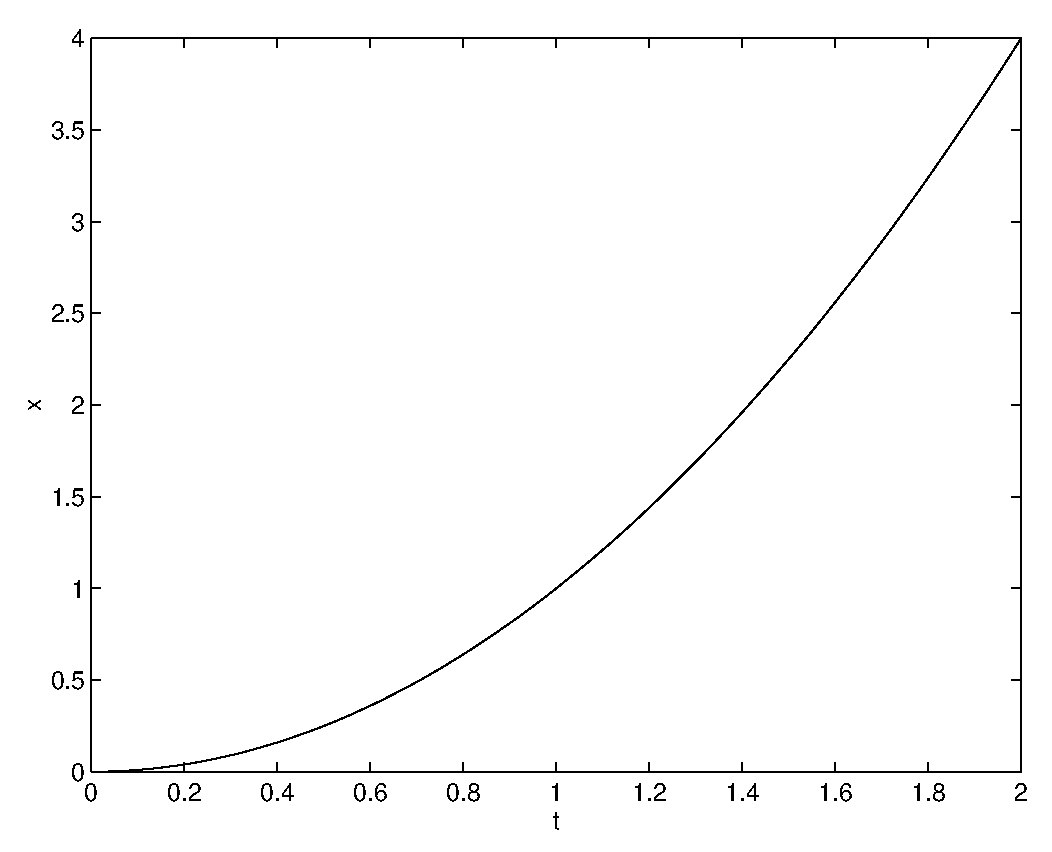
\psfig{file=exfigure/3-1-a78a.eps,width=1.35in}
                       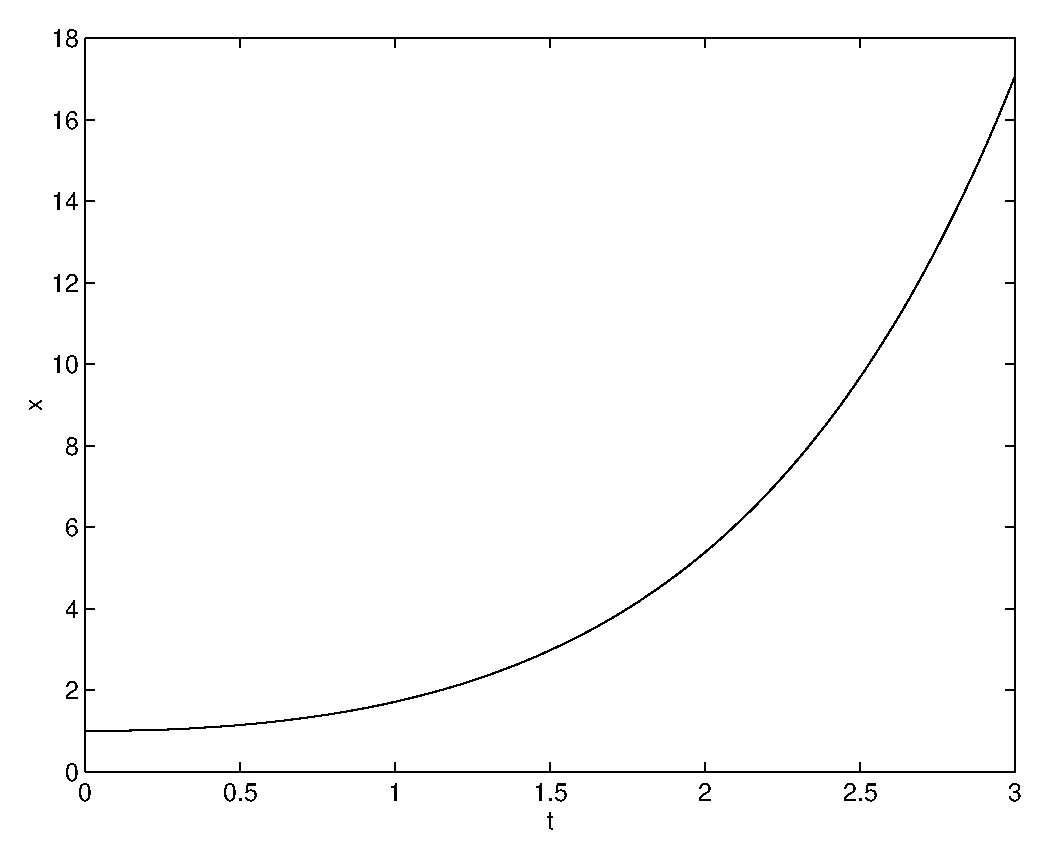
\psfig{file=exfigure/3-1-a78b.eps,width=1.35in}
                       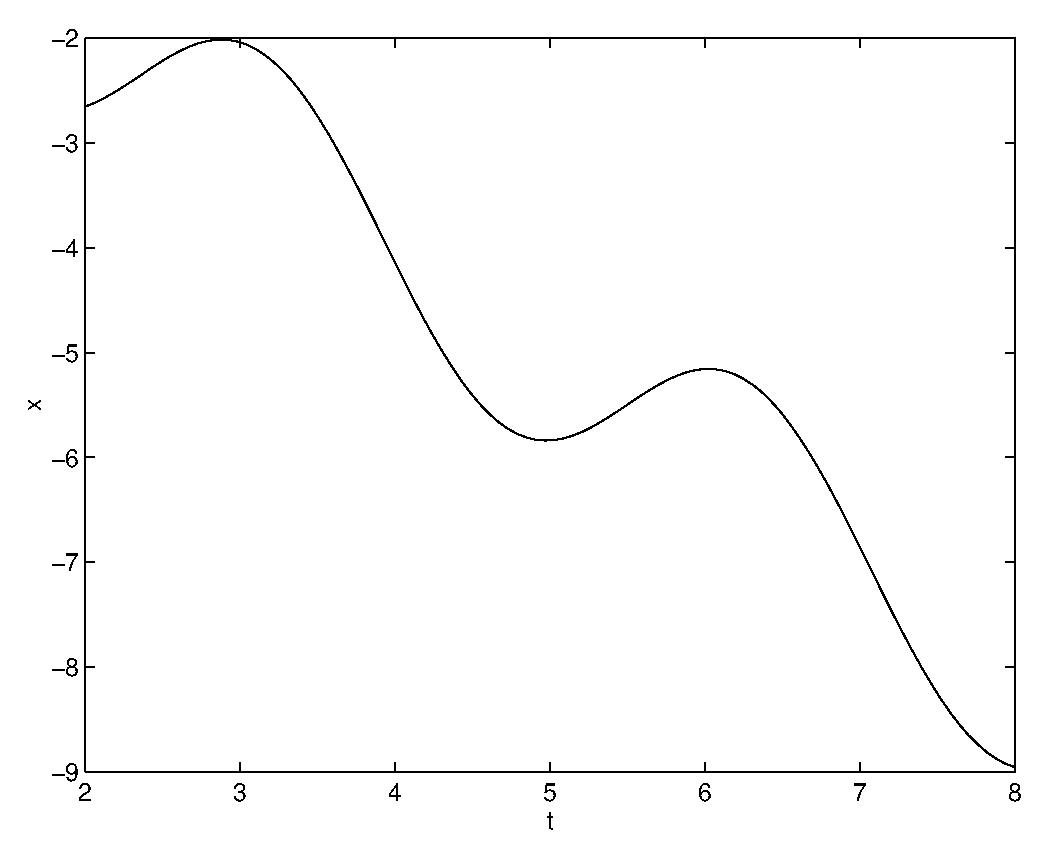
\psfig{file=exfigure/3-1-a78c.eps,width=1.35in}
                       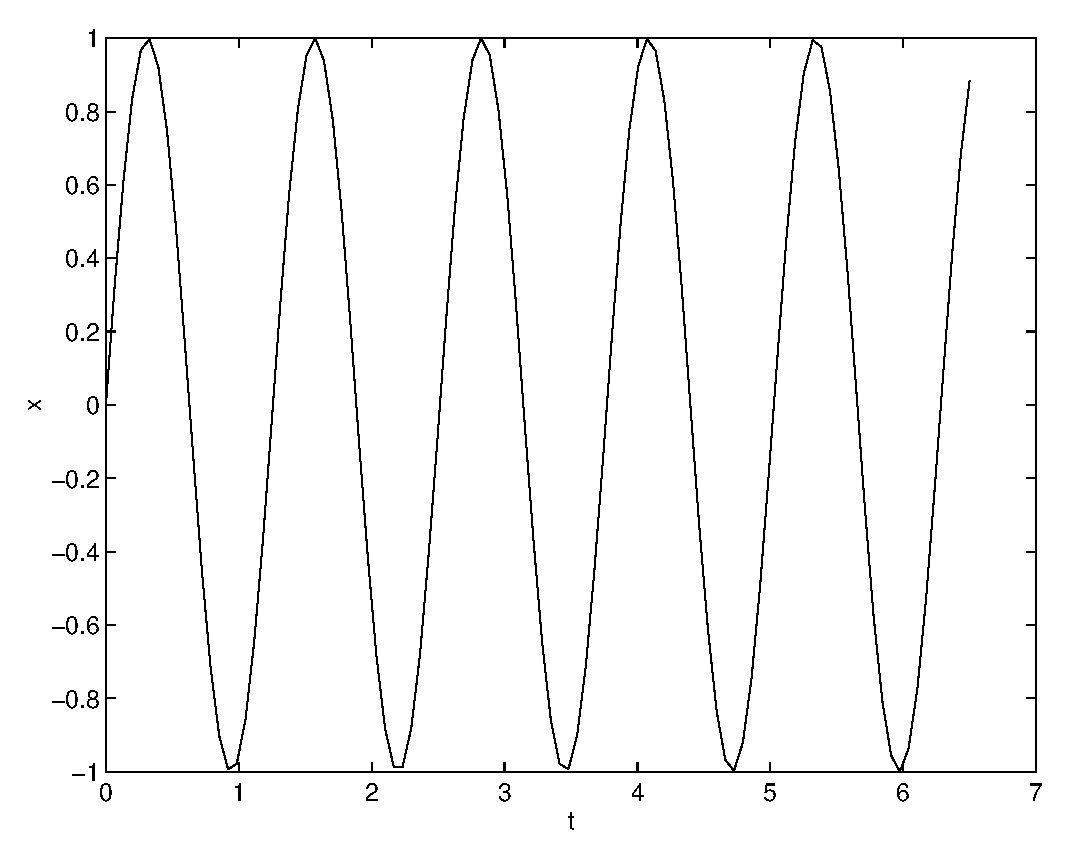
\psfig{file=exfigure/3-1-a78d.eps,width=1.35in}}
	\centerline{Figure~\ref{c3.1.a78a}\hspace{0.8in}
	Figure~\ref{c3.1.a78b}\hspace{0.8in}Figure~\ref{c3.1.a78c}
	\hspace{0.8in}Figure~\ref{c3.1.a78d}}
\end{figure}

\end{solution}
\end{exercise}

\noindent{\bf Hint:} Use the fact that the trigonometric functions $\sin$ and
$\cos$ can be evaluated in \Matlab in the same way as the exponential
function, that is, by using \verb+ sin + \index{\computer!sin} and
\verb+ cos + \index{\computer!cos} instead of \verb+ exp+.

\begin{exercise} \label{c3.1.8}
Two banks each pay $7\%$ interest per year --- one compounds money
daily and one compounds money continuously.  What is the difference
in earnings in one year in an account having \$10,000.

\begin{solution}

\ans The difference in earnings is 7 cents.

\soln Compute this using the interest
formula, since we are given that the principal $P_0 = \$10\mbox{,}000$,
the interest rate $r = 0.07$, and $t = 1$.  So we can substitute
these values into the interest formulas and find the amount of money
in each account after 1 year.  The formula for interest compounded daily is
\[ \begin{array}{rcl}
P(t) & = & P_0\left(1 + \frac{r}{365}\right)^{365t} \\
P(1) & = & \$10\mbox{,}000\left(1 + \frac{0.07}{365}\right)^{365} \\
P(1) & = & \$10\mbox{,}725.01\end{array}
\]
To find the amount of money in the account at the other bank, we substitute
into the formula for interest compounded instantaneously:
\[ \begin{array}{rcl}
P(t) & = & P_0e^{rt} \\
P(1) & = & \$10\mbox{,}000e^{0.07} \\
P(1) & = & \$10\mbox{,}725.08\end{array}
\]

\end{solution}
\end{exercise}

\begin{exercise} \label{c3.1.9}
There are two banks in town --- Intrastate and Statewide.  You plan
to deposit \$5,000 in one of these banks for two years.  Statewide Bank's
best savings account pays $8\%$ interest per year compounded quarterly
and charges \$10 to open an account.  Intrastate Bank's best savings
account pays $7.75\%$ interest compounded daily.  Which bank will
pay you the most money when you withdraw your money?  Would your
answer change if you had planned to keep your money in the bank
for only one year?

\begin{solution}

\ans After two years, an account at Statewide returns more interest than
the Intrastate account.  However, after only one year, the Intrastate
account returns more.

\soln To find the return from each account, use the formula for
compound interest:
\[
P(t) = P_0\left(1 + \frac{r}{N}\right)^{Nt}
\]
If you deposit your money at Statewide, $P_0 = \$4\mbox{,}990$ because of the
fine.  Interest is compounded four times a year, so $N = 4$.  The interest
rate is 8\%, so $r = 0.08$.
After two years, an account at Statewide returns
\[
P_{S}(2) = \$4\mbox{,}990\left(1 + \frac{0.08}{4}\right)^{2(4)} = 
\$5\mbox{,}846.58
\]
If you deposit your money at Intrastate, $r = 0.0775$.  Interest is
compounded daily, so $N = 365$.  So, after two years, the account returns
\[
P_{I}(2) = \$5\mbox{,}000\left(1 + \frac{0.0775}{365}\right)^{2(365)} = 
\$5\mbox{,}838.19.
\]
After only 1 year, however,
\[
P_{S}(1) = \$4\mbox{,}900\left(1 + \frac{0.08}{4}\right)^{4} = \$5\mbox{,}401.37
\]
at Statewide, and
\[
P_{I}(1) = \$5\mbox{,}000\left(1 + \frac{0.0775}{365}\right)^{365} = 
\$5\mbox{,}402.87
\]
at Intrastate.

\end{solution}
\end{exercise}

\begin{exercise} \label{c3.1.10}
In the beginning of the year 1990 the population of the United States was
approximately 250,000,000 people and the growth rate was estimated at $3\%$
per year.  Assuming that the growth rate does not change, during what year
will the population of the United States reach 400,000,000?

\begin{solution}

\ans According to this population model, the population of the United States
reaches 400,000,000 in the year 2005.

\soln Note that the population model represents a continuous growth
function $p(t) = p_0e^{rt}$.  Let $t$ be time in years, starting in 1990. 
So $p_0 = 250$ million.  The growth rate $r$ is $0.03$.  Thus, the
population at time $t$ (in millions) is $P(t) = 250e^{0.03t}$.
The population will reach 400,000,000 when $400 = 250e^{0.03t}$.
Solving for $t$ yields $t \approx 15.67$, that is, in the year 2005.



\end{solution}
\end{exercise}


\end{document}
